\documentclass[smaller]{beamer}
\usetheme[english]{Berlin}
\usepackage{ngerman}
\useoutertheme{infolines}
\beamertemplatenavigationsymbolsempty
\usepackage{pgfplots,tikz,subfigure}
\usepackage{amsmath,amsthm}
\usepackage{hyperref,graphics,graphicx,color,algorithm,algorithmic,enumerate}
\usepackage{mymacros,wrapfig,relsize}
\usepackage{pict2e}
\usepackage[utf8x]{inputenc}

\newcommand{\ri}{\mathrm{i}}
\newcommand{\T}{\mathsf{T}}
\renewcommand{\H}{\mathsf{H}}
\newcommand{\eps}{\varepsilon}
\newcommand{\To}{\rightarrow}
\newcommand{\sddots}{\scalebox{0.6}{$\ddots$}}
\usepackage[pdf]{pstricks}
\usepackage{sansmathfonts}
\usepackage{eurosym}
%\usepackage{arev}
%\renewcommand\familydefault{\sfdefault}

\DeclareMathOperator{\loc}{loc}
\DeclareMathOperator{\rank}{rank}
\DeclareMathOperator{\RE}{Re}
\DeclareMathOperator{\IM}{Im}
\DeclareMathOperator{\In}{In}
\DeclareMathOperator{\im}{im}
\DeclareMathOperator{\Gl}{Gl}
\DeclareMathOperator{\spa}{span}
\DeclareMathOperator{\ext}{{ext}}
\DeclareMathOperator{\ind}{ind}
\DeclareMathOperator{\normalrank}{normalrank}
\DeclareMathOperator{\essup}{ess\,sup}
\DeclareMathOperator{\vect}{vec}

\newcommand{\re}{\mathrm{e}}
\newcommand{\ddt}{\tfrac{\mathrm{d}}{\mathrm{d}t}}
\newcommand{\sys}[4]{\left[\begin{array}{c|c} #1 & #2 \\ \hline #3 & #4 \end{array}\right]}

\renewcommand{\tilde}{\widetilde}
\renewcommand{\hat}{\widehat}

\title[]{Optimierung f\"ur Studierende der Informatik}
\subtitle{-- 3. Vorlesung --}
\author[Matthias Voigt]{\textbf{Matthias Voigt$^{1,2}$}}
\institute[]{
\begin{columns}
%\begin{center}
\column{0.45\textwidth}{\centering {$^1$Universit\"at Hamburg \\ Fachbereich Mathematik \\ Hamburg \\ }}
\column{0.45\textwidth}{\centering {$^2$Technische Universit\"at Berlin \\ Institut f\"ur Mathematik \\ Berlin  \\}}
%\end{center}
\end{columns}
}
\date[]{Universit\"at Hamburg
\begin{columns}
\column{0.45\textwidth}{\centering \includegraphics[width = 1.2\textwidth]{uhh-logo.png}\\}
\end{columns}
}

\definecolor{tucgreen}{rgb}{0.0,0.5,0.27}
\definecolor{tucred}{rgb}{0.75,0,0}
\definecolor{tucorange}{rgb}{1.0,.5625,0}
\definecolor{mpired}{HTML}{990000}
\definecolor{mpigreen}{HTML}{5C871D}
\definecolor{mpiblue}{HTML}{006AA9}
\definecolor{mpibg1}{HTML}{5D8B8A}
\definecolor{mpibg2}{HTML}{BFDFDE}
\definecolor{mpibg3}{HTML}{A7C1C0}
\definecolor{mpibg4}{HTML}{7DA9A8}
\definecolor{mpigrey}{rgb}{0.9294,0.9294,0.8784}

\begin{document}

\maketitle

\begin{frame}
 \frametitle{Verbindungen zur Geometrie -- Polyeder}
 Im Zusammenhang mit der grafischen Methode hatten wir bereits Geraden, Halbebenen und Durchschnitte von endlich vielen Halbebenen im $\R^2$ betrachtet. Wir wollen einige der dort auftretenden Begriffe verallgemeinern. \\ \vspace*{0.2cm}
In der 1. Vorlesung hatten wir beispielsweise festgestellt: Sind $a_1,a_2,b \in \R$ gegeben und sind $a_1,a_2$ nicht beide gleich Null, so wird durch die Gleichung
\[
a_1x_1 + a_2x_2 = b
\]
eine \alert{Gerade im $\R^2$} dargestellt; die Menge aller Paare $(x_1,x_2) \in \R^2$, für die
\[
a_1x_1 + a_2x_2 \leq b
\]
gilt, bilden eine \alert{Halbebene}, die durch diese Gerade begrenzt wird.
\end{frame}

\begin{frame}
\frametitle{Ebenen und Halbr\"aume im $\R^3$}
\alert{Ähnliches gilt im $\R^3$}: Sind $a_1,a_2,a_3,b \in \R$ gegeben und sind $a_1,a_2,a_3$ nicht alle gleich Null, so wird durch die Gleichung 
\[
a_1x_1 + a_2x_2 + a_3x_3 = b
\]
eine \alert{Ebene im $\R^3$} dargestellt, und die Menge aller Tripel $(x_1,x_2,x_3) \in \R^3$, für die
\[
a_1x_1 + a_2x_2+a_3x_3 \leq b
\]
gilt, bilden einen \alert{Halbraum}, der durch diese Ebene begrenzt wird.
\end{frame}

\begin{frame}
 \frametitle{Hyperebenen und Halbr\"aume im $\R^n$}
 \alert{Analoge Sprechweisen verwendet man auch im $\R^n$}: Sind $a_1,\ldots,a_n,b \in \R^n$ gegeben und sind nicht alle $a_1,\ldots,a_n$ gleich Null, so nennt man die Menge aller $n$-Tupel $(x_1,\ldots,x_n) \in \R^n$, für die die Gleichung
\[
a_1x_1 + \ldots + a_nx_n = b
\]
gilt, eine \alert{Hyperebene im $\R^n$}; und die Menge aller $n$-Tupel $(x_1,\ldots,x_n) \in \R^n$, für die
\[
a_1x_1 + \ldots + a_nx_n \leq b
\]
gilt, nennt man einen \alert{Halbraum des $\R^n$}.
\end{frame}

\begin{frame}
 \frametitle{Ein Beispiel}
\textbf{Beispiel eines LP-Problems:}
\begin{align*}
\begin{alignedat}{5}
& \text{maximiere } & 3x_1 &\ + &\ 2x_2 &\ + &\ 5x_3 & & \\
& \rlap{unter den Nebenbedingungen} & & & & & & & \\
&& 2x_1 &\ + &\ x_2 &\  &\     &\ \leq &\ 4,\ \\
&&      &\   &\     &\  &\ x_3 &\ \leq &\ 5,\ \\
&& & & & & \llap{$x_1,x_2,x_3$} & \geq &\ 0.
\end{alignedat}
\end{align*}

Jede der fünf Nebenbedingungen beschreibt einen gewissen Halbraum des $\R^3$. Also ist die Menge der zulässigen Lösungen (der zulässige Bereich) dieses LP-Problems \alert{gleich dem Durchschnitt von fünf Halbräumen}. Eine derartige Menge bezeichnet man als \structure{Polyeder}. Genauer gilt: \\ \vspace*{0.2cm}
\textbf{Definition:}
Eine Teilmenge $P$ des $\R^n$ wird \textit{Polyeder} genannt, falls $P$ gleich dem Durchschnitt von endlich vielen Halbräumen des $\R^n$ ist oder falls $P = \R^n$ gilt.
\end{frame}

\begin{frame}
 \frametitle{Darstellung des Polyeders in unserem Beispiel}
 Das in unserem 3-dimensionalen Beispiel auftretende Polyeder ist in der folgenden Zeichnung dargestellt:
 \begin{center}
  \includegraphics{fig6.pdf}
 \end{center}
 In diesem Beispiel hat das Polyeder, das den Bereich der zulässigen Lösungen beschreibt, also die Gestalt eines \alert{Prismas}.
 
\end{frame}

\begin{frame}
 \frametitle{Flächen des Prismas}
 Zu jeder der fünf Begrenzungsflächen des Prismas gehört eine der fünf Nebenbedingungen. Genauer gilt: \alert{Die Punkte auf jeder der fünf Flächen\footnote{Statt {\glqq}Begrenzungsflächen{\grqq} sagt man häufig auch {\glqq}Seitenflächen{\grqq}. Wir werden hier der Einfachheit halber immer {\glqq}Flächen{\grqq} sagen.} erfüllen die zugehörige Nebenbedingung \textbf{mit Gleichheit}}. \\ \vspace*{0.2cm}
Beispielsweise entspricht die Grundfläche (der dreieckige Boden) der Nebenbedingung $x_3 \geq 0$: Für die Punkte auf dem Boden des Prismas gilt $x_3=0$. Der grauen Fläche auf der rechten Seite des Prismas entspricht die Nebenbedingung $2x_1+x_2 \leq 4$, und für die Punkte auf dieser Fläche gilt $2x_1+x_2 = 4$. 
\end{frame}

\begin{frame}
 \frametitle{Flächen und Nebenbedingungen}
 Die Entsprechungen zwischen Flächen einerseits und Nebenbedingungen andererseits werden besonders deutlich, wenn man \alert{Schlupfvariablen} $x_4$, $x_5$ wie üblich hinzunimmt. Es gelte also (Definition der Schlupfvariablen):
\begin{align*}
\begin{alignedat}{5}
x_4 &\ = &\ 4 &\ - &\ 2x_1 &\ - &\ x_2 &\   &      \\
x_5 &\ = &\ 5 &\   &\      &\   &\     &\ - &\ x_3.
\end{alignedat}
\end{align*}
\alert{Jeder Fläche des Polyeders entspricht dann genau eine der Variablen $x_1,\ldots,x_5$} in dem Sinne, dass $x_j=0$ für die Punkte auf der entsprechenden Fläche gilt. Im Einzelnen hat man Folgendes:
\begin{itemize}
\item für die Punkte auf der linken Fläche gilt $x_1=0$;
\item für die Punkte auf der Frontfläche gilt $x_2=0$;
\item für die Punkte auf der Grundfläche gilt $x_3=0$;
\item für die Punkte auf der grauen Fläche gilt $x_4=0$;
\item für die Punkte auf der oberen Fläche gilt $x_5=0$.
\end{itemize}
\end{frame}

\begin{frame}
 \frametitle{Zulässige Basislösungen -- Geometrische Deutung}
 Die Menge der zulässigen Lösungen haben wir bereits genau beschrieben: Es handelt sich um die Punkte des Prismas -- natürlich einschließlich derjenigen, die im Inneren des Prismas liegen. Insbesondere können wir festhalten, dass es unendlich viele zulässige Lösungen gibt. \alert{Die meisten dieser Lösungen werden -- wie wir wissen -- vom Simplexverfahren jedoch ignoriert}: Im Simplexverfahren kommen als Ergebnis einer Iteration nur \alert{zulässige Basislösungen} vor. \\ \vspace*{0.2cm}
 In jeder zulässigen Basislösung sind drei der fünf Variablen $x_1,\ldots,x_5$ Nichtbasisvariablen. Diese drei Variablen sind gleich Null, und die Werte der beiden übrigen Variablen sind dadurch eindeutig bestimmt, dass die Nichtbasisvariablen gleich Null gesetzt wurden. \alert{Geometrisch bedeutet dies, dass jeder Punkt, der eine zulässige Basislösung darstellt, ein eindeutig bestimmter Schnittpunkt von drei Flächen des Prismas ist}, dass es sich also um eine Ecke des Prismas handelt (vgl. Zeichnung).

%Statt Eckpunkt sagt man gewöhnlich auch \alert{Ecke} eines Polyeders.
\end{frame}

\begin{frame}
 \frametitle{Zulässige Basislösungen in unserem Beispiel}
 Wir wollen uns anschauen, was in unserem Beispiel geometrisch passiert, wenn wir es mit dem Simplexverfahren lösen. Wir interessieren uns vor allem für die \alert{zulässigen Basislösungen am Ende jeder Iteration}; außerdem geben wir an, welches am Ende jeder Iteration die Basisvariablen sind. Hier das Ergebnis: \\ \vspace*{0.2cm}

\underline{Startlösung}:
\[
x_1=0,\quad
x_2=0,\quad
x_3=0,\quad
x_4=4,\quad
x_5=5;\quad
\text{Basis: } x_4,\ x_5.
\]

\underline{Am Ende der 1. Iteration}:
\[
x_1=0,\quad
x_2=0,\quad
x_3=5,\quad
x_4=4,\quad
x_5=0;\quad
\text{Basis: } x_3,\ x_4.
\]

\underline{Am Ende der 2. Iteration}:
\[
x_1=2,\quad
x_2=0,\quad
x_3=5,\quad
x_4=0,\quad
x_5=0;\quad
\text{Basis: } x_1,\ x_3.
\]

\underline{Am Ende der 3. Iteration}:
\[
x_1=0,\quad
x_2=4,\quad
x_3=5,\quad
x_4=0,\quad
x_5=0;\quad
\text{Basis: } x_2,\ x_3.
\]
\end{frame}

\begin{frame}
 \frametitle{Entlang der Kanten zur optimalen Ecke}
 Am Ende der dritten Iteration wurde eine optimale Lösung erreicht: Im Punkt $(x_1,x_2,x_3) = (0,4,5)$ ist die Zielfunktion optimal (mit $z=33$). Auf dem Weg zu diesem Ergebnis erhielten wir die obigen zulässigen Basislösungen; die dazugehörigen Punkte waren:
\begin{align*}
(x_1,x_2,x_3) &= (0,0,0), \\
(x_1,x_2,x_3) &= (0,0,5), \\
(x_1,x_2,x_3) &= (2,0,5), \\
\intertext{sowie schließlich}
(x_1,x_2,x_3) &= (0,4,5). \\
\end{align*}

Es handelt sich dabei -- wie aufgrund unserer Vorüberlegungen nicht anders zu erwarten war -- um \alert{Ecken unseres Prismas} (siehe obige Zeichnung). \alert{Die Übergänge von einer Ecke zur nächsten lassen sich als kontinuierliche Bewegung längs der Kanten interpretieren}.
\end{frame}

\begin{frame}
 \frametitle{Entlang der Kanten zur optimalen Ecke}
 Betrachten wir beispielsweise die 2. Iteration: Eingangsvariable war hier $x_1$. Die aktuelle Ecke vor der 2. Iteration war $(0,0,5)$. Nach Wahl von $x_1$ als Eingangsvariable wurde der Wert von $x_1$ kontinuierlich angehoben -- unter Beibehaltung von $x_2=0$ und $x_5=0$. Die Bedingung $x_2=x_5=0$ besagt, dass wir nur Punkte betrachten, die sowohl zur vorderen als auch zur oberen Fläche des Polyeders gehören. (Man beachte: $x_2=0$ ist die Bedingung für die vordere, $x_5=0$ die Bedingung für die obere Fläche.) \\ \vspace*{0.2cm}

Beim Anheben von $x_1$ unter Beibehaltung von $x_2=0$ und $x_5=0$ bewegen wir uns also längs der Kante, die sowohl zur vorderen als auch zur oberen Fläche gehört -- und zwar solange, bis wir die nächste Ecke erreicht haben. \alert{In unserem Fall haben wir uns also von $(0,0,5)$ zu $(2,0,5)$ bewegt}.
\end{frame}

\begin{frame}
 \frametitle{Typischer Ablauf des Simplexverfahrens}
 Wir haben in unserem Beispiel \alert{den typischen Ablauf des Simplexverfahrens} geometrisch beschrieben. \\ \vspace*{0.2cm}
\textbf{Feststellung:} 
\begin{itemize}
\item Kommen keine degenerierten Iterationen vor, \alert{so bewegt man sich längs bestimmter Kanten des zugehörigen Polyeders von einer Ecke zur nächsten, wobei der Zielfunktionswert steigt.} 
\item \alert{Man stoppt, wenn man an einer optimalen Ecke angekommen ist} bzw. wenn man feststellt, dass das Problem unbeschränkt ist.
\end{itemize}

Bei dieser Beschreibung haben wir vorausgesetzt, dass das Problem lösbar ist und dass wir ein Starttableau kennen (und somit auch eine \alert{Startecke}). Falls degenerierte Iterationen auftreten, so ändert sich an der Beschreibung nicht viel: Es kann dann zusätzlich vorkommen, dass man auf einer Ecke verweilt. (Zur Erinnerung: Bei einer degenerierten Iteration ändert sich nur die Basis, die zulässige Basislösung ändert sich nicht.)
\end{frame}

\begin{frame}
 \frametitle{Wie schnell ist das Simplexverfahren?}
 Aus empirischen Untersuchungen wissen wir für in der Praxis auftretende LP-Probleme mit $n$ Entscheidungsvariablen und $n+m$ Nebenbedingungen:
 \begin{itemize}
 \item Wir benötigen häufig weniger als $\frac{3}{2}m$ Iterationen -- und nur sehr selten werden mehr als $3m$ Iterationen benötigt. 
 \item Außerdem wird der folgende empirische Befund erwähnt (siehe Chvátal, Kapitel 4): Bei festem $m$ und wachsendem $n$ nimmt die Anzahl der Iterationen nur sehr langsam zu; es wurde ein Wachstum ungefähr von der Größenordnung $\log(n)$ beobachtet.
\end{itemize}
 \alert{Die Ergebnisse dieser empirischen Untersuchungen stehen im Einklang mit der Tatsache, \textbf{dass sich das Simplexverfahren seit mehr als 60 Jahren in der Praxis hervorragend bewährt hat}}.
\end{frame}
 
\begin{frame}
 \frametitle{Regel vom größten Koeffizienten}
 \alert{Auf der anderen Seite sind aber auch Beispiele bekannt, die eine außerordentlich hohe Anzahl von Iterationen erfordern}. Derartige Beispiele wurden erstmals im Jahre 1972 in einer Arbeit von Klee und Minty vorgestellt. Bevor wir uns dieses Beispiel anschauen, sei an eine Pivotierungsregel erinnert, die wir bereits häufig verwendet haben: \\ \vspace*{0.2cm}
%\begin{equation}
%\label{eq:5:*}
%\tag{$\star$}
\begin{quote}
{Stehen mehrere Kandidaten für die Wahl einer Eingangsvariable} 
{zur Verfügung, so entscheide man sich für eine Variable, deren Koeffizient $\overline{c}_j$ } 
{in der $z$-Zeile des aktuellen Tableaus \alert{möglichst groß} ist.}
\end{quote}
%\end{equation}

Diese Regeln nennt man die \structure{Regel vom größten Koeffizienten}.

Auch im Folgenden soll immer, wenn nichts anderes gesagt ist, die Regel vom größten Koeffizienten zugrunde liegen.
\end{frame}

\begin{frame}
 \frametitle{Beispiele von Klee und Minty}
 Hier sind nun die \textbf{Beispiele von Klee und Minty}:
\begin{align*}
\begin{alignedat}{5}
& \text{maximiere } & \sum\limits_{j=1}^{n}{10^{n-j}x_j} & & & & & \\
& \rlap{unter den Nebenbedingungen} & & & & & & \\
&& 2 \cdot \sum\limits_{j=1}^{i-1}{10^{i-j}x_j} &\ + &\ x_i &\ \leq &\ 100^{i-1} & \qquad (i=1,\ldots,n), \\
&&                                              &    &\ x_j &\ \geq &\         0 & \qquad (j=1,\ldots,n).
\end{alignedat}
\end{align*}

Klee und Minty haben in ihrer Arbeit nachgewiesen, dass für dieses Beispiel \alert{$2^n-1$ Iterationen} nötig sind, bis das Simplexverfahren terminiert (bei Anwendung der Regel vom größten Koeffizienten).
\end{frame}

\begin{frame}
 \frametitle{Beispiele von Klee und Minty für $n=3$}
 Wir schauen uns den Fall $n=3$ näher an:
\begin{align*}
\begin{alignedat}{5}
& \text{maximiere } & 100x_1 &\ + &\ 10x_2 &\ + &\ x_3 & & \\
& \rlap{unter den Nebenbedingungen} & & & & & & & \\
&&    x_1 &\   &\       &\   &\     &\ \leq &\     1,\ \\
&&  20x_1 &\ + &\   x_2 &\   &\     &\ \leq &\   100,\ \\
&& 200x_1 &\ + &\ 20x_2 &\ + &\ x_3 &\ \leq &\ 10000,\ \\
&& & & & & \llap{$x_1,x_2,x_3$}     &\ \geq &\     0.\
\end{alignedat}
\end{align*}

Unter Benutzung der Regel vom größten Koeffizienten erhalten wir die folgenden Tableaus: \\ \vspace*{0.2cm}

\textbf{Starttableau:}
\begin{align*}
\begin{alignedat}{5}
x_4 &\ = &\     1 &\ - &\    x_1, &\   &\       &\   &\      \\
x_5 &\ = &\   100 &\ - &\  20x_1\ &\ - &\   x_2, &\   &\      \\
x_6 &\ = &\ 10000 &\ - &\ 200x_1\ &\ - &\ 20x_2\ &\ - &\ x_3,\ \ \\ \cline{1-9}
  z &\ = &\       &\   &\ 100x_1\ &\ + &\ 10x_2\ &\ + &\ x_3. 
\end{alignedat}
\end{align*}
\end{frame}

\begin{frame}
 \frametitle{Die 1. und 2. Iteration}
 Nach der \textbf{1. Iteration} ergibt sich:
\begin{align*}
\begin{alignedat}{5}
x_1 &\ = &\     1 &\ - &\    x_4, &\   &\       &\   &\      \\
x_5 &\ = &\    80 &\ + &\  20x_4\ &\ - &\   x_2, &\   &\      \\
x_6 &\ = &\  9800 &\ + &\ 200x_4\ &\ - &\ 20x_2\ &\ - &\ x_3,\ \\ \cline{1-9}
  z &\ = &\   100 &\ - &\ 100x_4\ &\ + &\ 10x_2\ &\ + &\ x_3.\  
\end{alignedat}
\end{align*}

Nach der \textbf{2. Iteration} ergibt sich:
\begin{align*}
\begin{alignedat}{5}
x_1 &\ = &\     1 &\ - &\    x_4, &\   &\       &\   &\      \\
x_2 &\ = &\    80 &\ + &\  20x_4\ &\ - &\   x_5, &\   &\      \\
x_6 &\ = &\  8200 &\ - &\ 200x_4\ &\ + &\ 20x_5\ &\ - &\ x_3,\ \\ \cline{1-9}
  z &\ = &\   900 &\ + &\ 100x_4\ &\ - &\ 10x_5\ &\ + &\ x_3.\  
\end{alignedat}
\end{align*}
\end{frame}

\begin{frame}
 \frametitle{Die 3. und 4. Iteration}
 Nach der \textbf{3. Iteration} ergibt sich:
\begin{align*}
\begin{alignedat}{5}
x_4 &\ = &\     1 &\ - &\    x_1, &\   &\       &\   &\      \\
x_2 &\ = &\   100 &\ - &\  20x_1\ &\ - &\   x_5, &\   &\      \\
x_6 &\ = &\  8000 &\ + &\ 200x_1\ &\ + &\ 20x_5\ &\ - &\ x_3,\ \\ \cline{1-9}
  z &\ = &\  1000 &\ - &\ 100x_1\ &\ - &\ 10x_5\ &\ + &\ x_3.\  
\end{alignedat}
\end{align*}

Nach der \textbf{4. Iteration} ergibt sich:
\begin{align*}
\begin{alignedat}{5}
x_4 &\ = &\     1 &\ - &\    x_1, &\   &\       &\   &\      \\
x_2 &\ = &\   100 &\ - &\  20x_1\ &\ - &\   x_5, &\   &\      \\
x_3 &\ = &\  8000 &\ + &\ 200x_1\ &\ + &\ 20x_5\ &\ - &\ x_6,\ \\ \cline{1-9}
  z &\ = &\  9000 &\ + &\ 100x_1\ &\ + &\ 10x_5\ &\ - &\ x_6.\  
\end{alignedat}
\end{align*}
\end{frame}

\begin{frame}
 \frametitle{Die 5. und 6. Iteration}
 Nach der \textbf{5. Iteration} ergibt sich:
\begin{align*}
\begin{alignedat}{5}
x_1 &\ = &\     1 &\ - &\    x_4, &\   &\       &\   &\      \\
x_2 &\ = &\    80 &\ + &\  20x_4\ &\ - &\   x_5, &\   &\      \\
x_3 &\ = &\  8200 &\ - &\ 200x_4\ &\ + &\ 20x_5\ &\ - &\ x_6,\ \\ \cline{1-9}
  z &\ = &\  9100 &\ - &\ 100x_4\ &\ + &\ 10x_5\ &\ - &\ x_6.\ 
\end{alignedat}
\end{align*}

Nach der \textbf{6. Iteration} ergibt sich:
\begin{align*}
\begin{alignedat}{5}
x_1 &\ = &\     1 &\ - &\    x_4, &\   &\       &\   &\      \\
x_5 &\ = &\    80 &\ + &\  20x_4\ &\ - &\   x_2, &\   &\      \\
x_3 &\ = &\  9800 &\ + &\ 200x_4\ &\ - &\ 20x_2\ &\ - &\ x_6,\ \\ \cline{1-9}
  z &\ = &\  9900 &\ + &\ 100x_4\ &\ - &\ 10x_2\ &\ - &\ x_6.\  
\end{alignedat}
\end{align*}
\end{frame}

\begin{frame}
 \frametitle{Die 7. Iteration}
 Nach der 7. Iteration ergibt sich:
\begin{align*}
\begin{alignedat}{5}
x_4 &\ = &\     1 &\ - &\    x_1, &\   &\       &\   &\      \\
x_5 &\ = &\   100 &\ - &\  20x_1\ &\ - &\   x_2, &\   &\      \\
x_3 &\ = &\ 10000 &\ - &\ 200x_1\ &\ - &\ 20x_2\ &\ - &\ x_6\ \\ \cline{1-9}
  z &\ = &\ 10000 &\ - &\ 100x_1\ &\ - &\ 10x_2\ &\ - &\ x_6.\  
\end{alignedat}
\end{align*}

\textbf{Beobachtung}: Hätten wir in der 1. Iteration nicht $x_1$, sondern $x_3$ als Eingangsvariable gewählt, so wären wir schon nach einem Schritt fertig gewesen. \alert{Es stellt sich also unter anderem die Frage nach alternativen Pivotierungsregeln}.
\end{frame}

\begin{frame}
 \frametitle{Alternative Pivotierungsregeln}
 Besonders naheliegend ist die folgende Pivotierungsregel, die man die \alert{Regel vom größten Zuwachs} nennt. Nach dieser Regel wird der Kandidat für die Aufnahme in die Basis so gewählt, dass ein möglichst großer Zuwachs der Zielfunktion $z$ dabei herauskommt. \\ \vspace*{0.2cm}

Während die Regel vom größten Koeffizienten sehr einfach zu handhaben ist, ist die Regel vom größten Zuwachs deutlich rechenaufwendiger. \\ \vspace*{0.2cm}

Außerdem gilt (was auf den ersten Blick etwas überraschend sein mag): \alert{Auch für die Regel vom größten Zuwachs lassen sich Beispiele angeben, die in Bezug auf diese Regel eine ähnliche Rolle spielen, wie die Klee-Minty-Beispiele für die Regel vom größten Koeffizienten}. Derartige Beispiele wurden 1973 von R. G. Jeroslow vorgestellt.
\end{frame}

\begin{frame}
 \frametitle{Weitere Pivotierungsregeln}
 Eine weitere Pivotierungsregel ist uns bereits in der letzten Vorlesung begegnet: die \alert{Regel vom kleinsten Index (Blandsche Regel)}. \\ \vspace*{0.2cm}

Weitere Pivotierungsregeln werden im Buch von Matou\v{s}ek und Gärtner diskutiert. Für alle dort aufgeführten Regeln (einschließlich der Blandschen Regel) gilt: Es existieren Beispiele, die (ähnlich wie die Klee-Minty-Beispiele) zu einer außerordentlich hohen Zahl von Iterationen führen. Vielfach ist versucht worden, eine Pivotierungsregel zu finden, für die dies nicht der Fall ist -- bislang ohne Erfolg. \\ \vspace*{0.2cm}
\begin{quote}
\alert{\textbf{Offenes Problem:} Gibt es eine Pivotierungsregel, durch die das Simplexverfahren zu einem polynomiellen Algorithmus wird?}
\end{quote}

\alert{Diese Bemerkungen stehen im Übrigen keineswegs im Widerspruch zu der Tatsache, dass sich die Simplexmethode in der Praxis hervorragend bewährt hat: Die Beispiele zeigen ja nur, dass \textbf{im schlechtesten Fall} außerordentlich viele Iterationen nötig sind}.
\end{frame}

\begin{frame}
 \frametitle{Weitere Algorithmen für LP-Probleme}
 Keine der bekannten Pivotierungsregeln führt zu einem Algorithmus mit polynomieller Laufzeit. \\ \vspace*{0.2cm}
 Es war lange Zeit offen, ob ein solcher Algorithmus zur Lösung von LP-Problemen überhaupt existiert -- bis \alert{L.~G.~Khachiyan} im Jahre 1979 einen polynomiellen Algorithmus zur Lösung von LP-Problemen vorstellte, der unter dem Namen \structure{Ellipsoid-Methode} bzw. als \structure{Khachiyan-Algorithmus} bekannt wurde. Das war damals eine Sensation, über die sogar die New York Times auf ihrer ersten Seite berichtete. \\ \vspace*{0.2cm}
 Ein weiterer Algorithmus mit polynomieller Laufzeit wurde ca. 5 Jahre später von \alert{N. Karmarkar} vorgestellt; der Algorithmus von Karmarkar stellt ein Beispiel einer ganzen Klasse von Algorithmen zur Lösung von LP-Problemen dar, die man \structure{Innere-Punkte-Algorithmen} nennt.
\end{frame}

\begin{frame}
 \frametitle{Fazit}
 \textbf{Fazit:}
\begin{quote}
\alert{Ein lineares Programm ist sowohl in der Theorie als auch Praxis lösbar.}
\end{quote}

\begin{itemize}
\item \alert{In der Praxis} sind zahlreiche Softwarepakete verfügbar. Diese können Probleme mit mehreren Tausend Entscheidungsvariablen und Nebenbedingungen lösen. Lineare Programme mit spezieller Struktur (z.\,B. dünnbesetzte Probleme, bei denen die Matrix $A$ der Nebenbedingungen nur wenige Nichtnulleinträge besitzt), können sogar für viel höhere Dimensionen behandelt werden.

\item \alert{In der Theorie} wurden Algorithmen entwickelt, die jedes lineare Programm in beweisbar polynomieller Zeit in Abhängigkeit der {\glqq}Größe{\grqq} der Eingabedaten lösen können. Die {\glqq}Größe{\grqq} der Eingabedaten bezieht sich auf die Gesamtzahl der Bits, die benötigt werden, um alle Koeffizienten der Zielfunktion und der Nebenbedingungen zu speichern. 
\end{itemize}

%These two statements summarize the results of long and strenuous research, and efficient methods for linear programming are not simple.
 
\end{frame}

\begin{frame}
 \frametitle{Beispiele aus unterschiedlichen Lehrbüchern}
 Bevor wir nun mit dem zentralen Thema \alert{Dualität} fortfahren, wollen wir einen \alert{Eindruck von den vielfältigen Einsatz- und Anwendungsmöglichkeiten der linearen Programmierung} gewinnen. \\ \vspace*{0.2cm}

Zu diesem Zweck schauen wir uns Beispiele aus verschiedenen Lehrbüchern an.
 
\end{frame}

\begin{frame}
 \frametitle{Beispiele aus unterschiedlichen Lehrbüchern}
 In der \alert{1. Vorlesung} haben wir als einführendes Beispiel ein \alert{Diätproblem} betrachtet, das Ihnen möglicher\-weise etwas speziell vorkam. \\ \vspace*{0.2cm}

\alert{Das Problem ist jedoch weit weniger speziell, als es auf den ersten Blick erscheint}: Viele Probleme aus der Praxis, die gar nichts mit gesunder oder preiswerter Ernährung zu tun haben, entpuppen sich bei genauerem Hinsehen ebenfalls als {\glqq}Diätprobleme{\grqq}. Um dies zu erkennen, betrachten wir das folgende Beispiel, das wir \alert{das (allgemeine) Diätproblem} nennen\footnote{Dieses Beispiel stammt aus D. Luenberger, Yinyu Ye: \textit{Linear and Nonlinear Programming}. Springer (2008, 3. Auflage).}.
\end{frame}

\begin{frame}
 \frametitle{Das allgemeine Diätproblem}
 \textbf{Beispiel 1:} Wie können wir den ökonomisch preiswertesten Ernährungsplan unter Berücksichtigung gewisser Mindestanforderungen an die Ernährung bestimmen? Ein derartiges Problem kann beispielsweise bei Großküchen auftreten, die möglichst preiswert produzieren müssen. Wir nehmen an, dass auch dem Markt $n$ Lebensmittel gibt und dass das $j$-te Lebensmittel zum Preis $c_j$ pro Einheit verfügbar ist. Zudem gibt es $m$ grundlegende Nährstoffe -- für eine ausgewogene Ernährung sollte man $b_i$ Einheiten des $i$-ten Nährstoffs pro Tag aufnehmen. Wir nehmen zudem an, dass jede Einheit des $j$-ten Lebensmittels $a_{ij}$ Einheiten des $i$-ten Nährstoffs enthält.
\end{frame}

\begin{frame}
 \frametitle{Das allgemeine Diätproblem}
 Falls wir mit $x_j$ die Anzahl der Einheiten des $j$-ten Lebensmittels im Ernährungsplan bezeichnen, so besteht das Problem darin, die $x_j$ so zu wählen, dass die Gesamtkosten
\[
c_1x_1 + \ldots + c_nx_n 
\]
minimiert werden, unter den Nebenbedingungen

\begin{align*}
\begin{alignedat}{4}
a_{11}x_1 &\ + &\ \ldots &\ + &\ a_{1n}x_n &\ \geq &\ b_1, \\
 & & & \ \ \vdots & & & \\
a_{m1}x_1 &\ + &\ \ldots &\ + &\ a_{mn}x_n &\ \geq &\ b_m, 
\end{alignedat}
\end{align*}
und den Nichtnegativitätsbedingungen
\[
x_1 \geq 0, \ldots, x_n \geq 0.
\]
\end{frame}

\begin{frame}
 \frametitle{Diätprobleme mit und ohne obere Schranken}
 Ein Unterschied zwischen dem allgemeinen Diätproblem und Pauls Problem aus der 1. Vorlesung fällt auf: In Pauls Problem gab es obere Schranken für jedes Lebensmittel; im Einzelnen lauten diese:
\begin{align*}
x_1 &\leq 4 \\
x_2 &\leq 3 \\
x_3 &\leq 2 \\
x_4 &\leq 8 \\
x_5 &\leq 2 \\
x_6 &\leq 2.
\end{align*}

Im allgemeinen Diätproblem kommen dagegen keine oberen Schranken vor; deshalb wollen wir zwischen den folgenden Problemen unterscheiden:
\begin{itemize}
\item dem allgemeinen \structure{Diätproblem} (d.h. ohne obere Schranken),
\item dem allgemeinen \structure{Diätproblem mit oberen Schranken}.
\end{itemize}
 
\end{frame}

\begin{frame}
 \frametitle{Zusammenhang zwischen den beiden Varianten}
 Um zu erläutern, welcher Zusammenhang zwischen diesen beiden Varianten des Diätproblems besteht, betrachten wir noch einmal das Beispiel von Paul und seinen Lebensmitteln. \\ \vspace*{0.2cm}

Wir stellen uns vor, dass Paul sein Problem \alert{zunächst ohne obere Schranken} formuliert und auch gelöst hat (per Hand oder mithilfe eines der gängigen Softwarepakete). Möglicherweise wäre er dann mit dem Ergebnis nicht zufrieden gewesen, da der Speiseplan zu einseitig ausgefallen wäre. Um dies zu ändern, würde Paul dann \alert{nachträglich} die zusätzlichen Nebenbedingungen hinzunehmen.
\end{frame}

\begin{frame}
 \frametitle{Nachträgliche Hinzunahme von Nebenbedingungen}
 \alert{Die nachträgliche Hinzunahme von zusätzlichen Nebenbedingungen ist nichts Seltenes} -- im Gegenteil:
 \begin{quote}
 \alert{Es handelt sich um einen typischen Vorgang, der in der Praxis häufig vorkommt}.
 \end{quote}
 
 Das liegt daran, dass bei der Lösung eines LP-Problems natürlich nur diejenigen Nebenbedingungen Berücksichtigung finden, die explizit formuliert wurden. Das kann dazu führen, dass ein Anwender mit dem Ergebnis unzufrieden ist, da er noch zusätzliche Nebenbedingungen im Hinterkopf hatte. Dann kommt es darauf an, geeignete zusätzliche Nebenbedingungen explizit zu formulieren und einen weiteren Durchlauf zu starten.
\end{frame}

\begin{frame}
 \frametitle{Energieflussproblem}
 Das nachfolgende Beispiel übernehmen wir aus
\begin{itemize}
\item K. Neumann, M. Morlock: \textit{Operations Research}. Hanser-Verlag (2004, 2. Auflage).
\end{itemize}

Bei einem Problem der Versorgung mit elektrischer Energie soll von einer Quelle $V_0$ (Kraftwerk) über ein Leitungsnetz mit den Verteilerknoten (Umspannwerken) $V_1, \ldots, V_7$ die Senke $V_8$ (Fabrik) bedient werden. 

\begin{center}
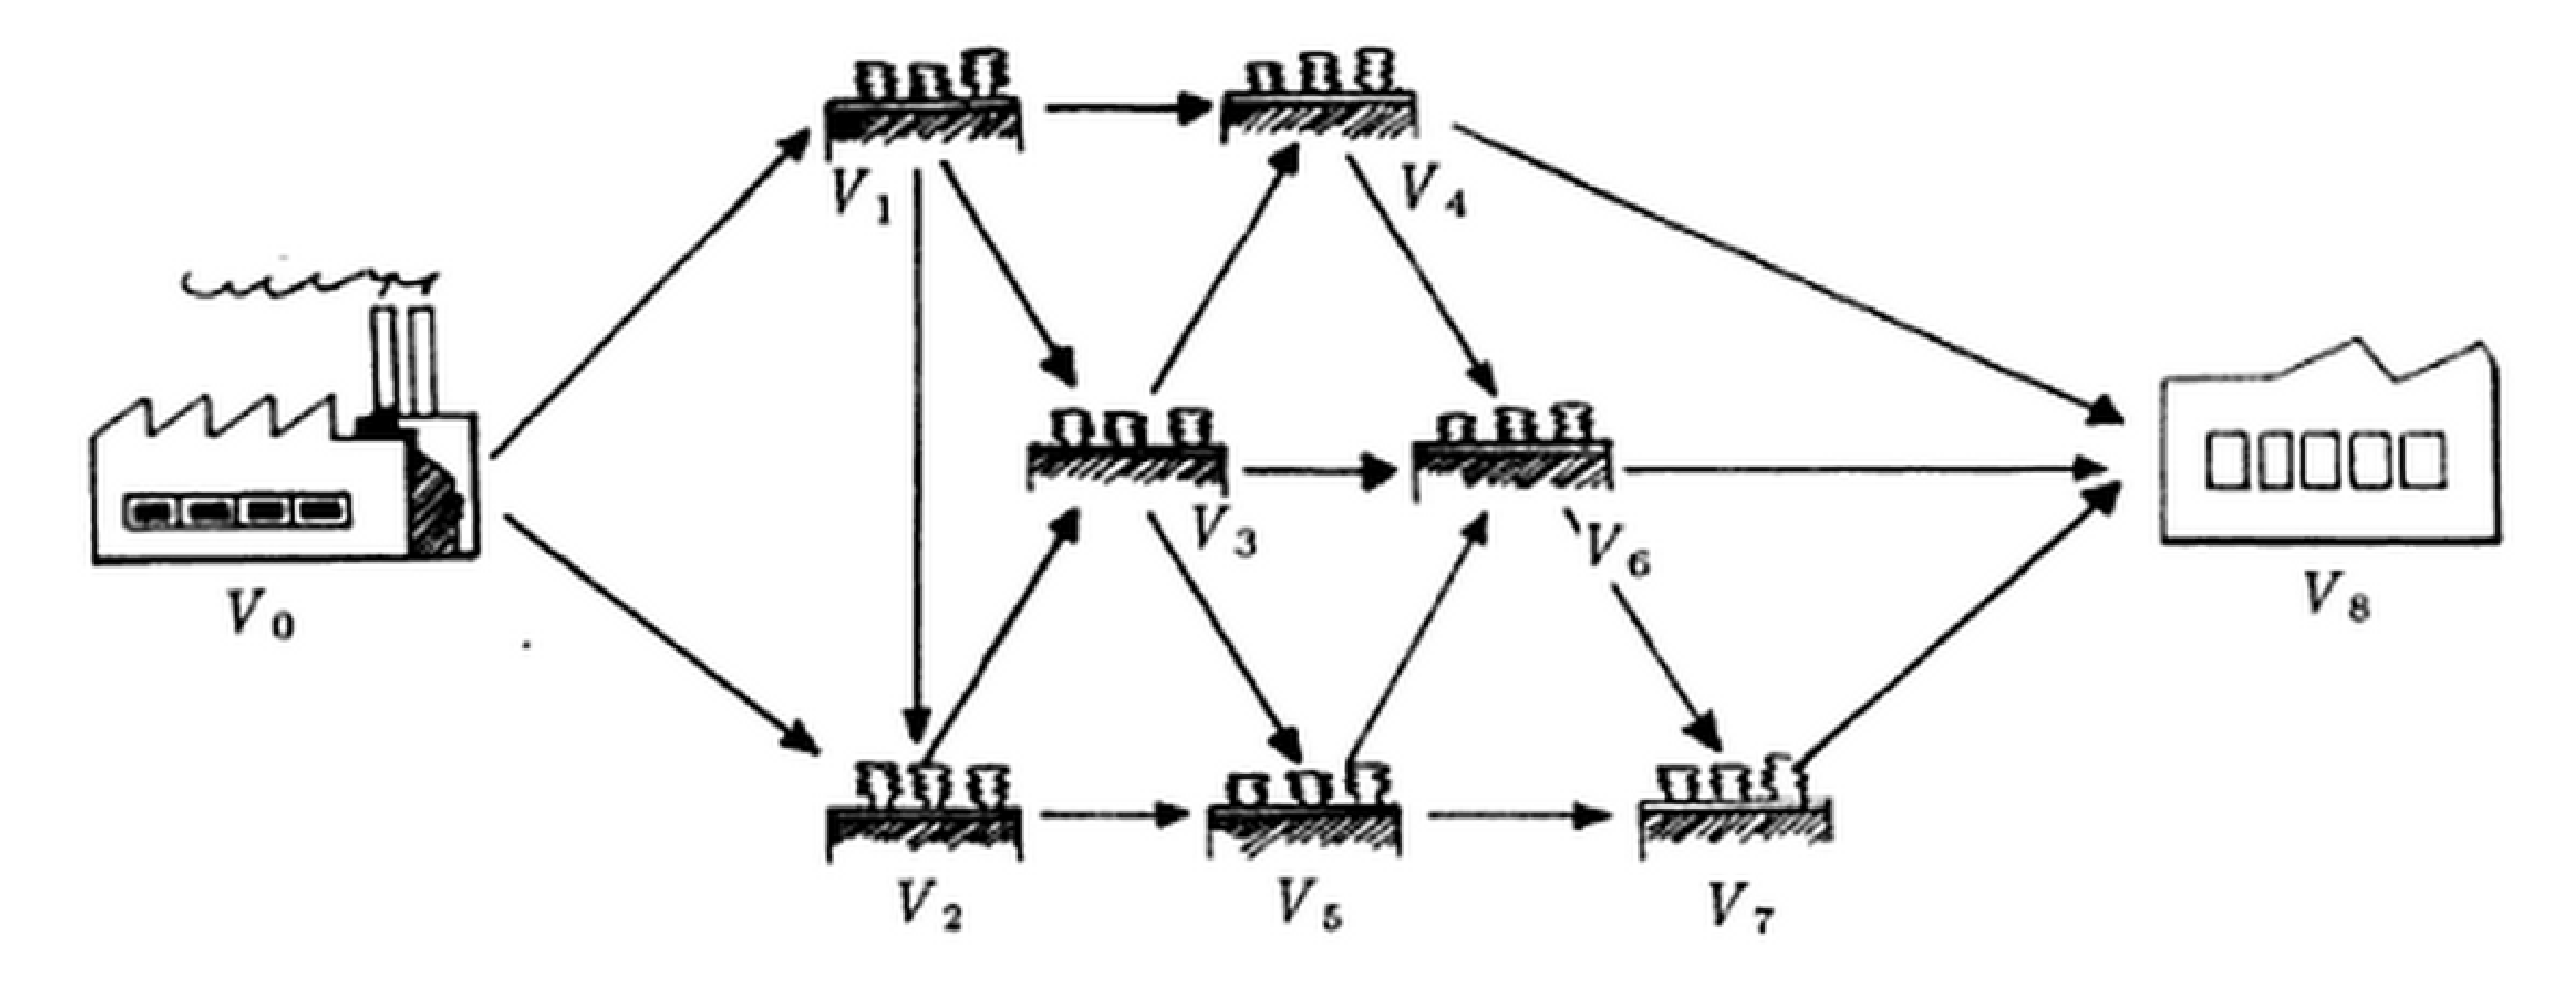
\includegraphics[width=0.8\textwidth]{energiefluss}
\end{center}
\end{frame}

\begin{frame}
 \frametitle{Zwei Optimierungsprobleme}
 Weder in den Verteilerknoten noch in den Leitungen gehe Elektrizität verloren, d.h., der gesamte in $V_0$ eingespeiste Strom wird in $V_8$ abgenommen. \\ \vspace*{0.2cm}
 Berücksichtigt man für die Leitungen Maximalbelastungen, so besteht eine Optimierungsaufgabe darin, die größtmögliche Strommenge zu bestimmen, die $V_8$ erreichen kann. \\ \vspace*{0.2cm}
 Ein anderes Optimierungsproblem ergibt sich, wenn elektrischer Strom einer vorgegebenen Stärke kostenoptimal durch ein Netz (von der Quelle zur Senke) geschickt werden soll und die Kosten aus Spannungsverlusten resultieren, die jeweils proportional zu den Stromstärken in den Leitungen sind.
\end{frame}

\begin{frame}
 \frametitle{Knotenbedingungen}
 Bezeichnen wir mit $x_{ij}$ den von $V_i$ nach $V_j$ fließenden Strom\footnote{Genauer: Unter der Voraussetzung, dass die Kante von $v_i$ nach $v_j$ vorhanden ist, bezeichnen wir mir $x_{ij}$ den über diese Kante von $v_i$ nach $v_j$ fließenden Strom.}, so erhalten wir neben einer Zielfunktion in der bekannten linearen Form für jeden Verteilerknoten die Bedingung, dass die hineinfließende gleich der herausfließenden Menge ist. Beispielsweise gilt für $V_3$
\[
x_{13} + x_{23} - x_{34} - x_{35} - x_{36} = 0.
\]

Eine entsprechende Beziehung gilt für die Quelle und die Senke. Die aus der Quelle herausfließende Menge $w$ ist gerade gleich der in die Senke hineinfließenden Menge, da in den Verteilerknoten nichts {\glqq}{verlorengeht}{\grqq}. Für das obige Beispiel erhalten wir damit
\[
x_{01} + x_{02} = w = x_{48} + x_{68} + x_{78}.
\]
\end{frame}

\begin{frame}
 \frametitle{Kapazitätsschranken}
 Neben diesen sogenannten \structure{Knotenbedingungen} sind noch die Maximalbelastungen der Leitungen als \structure{(obere) Kapazitätsschranken} zu beachten, d.h., für die Stärke $x_{ij}$ des von $V_i$ nach $V_j$ fließenden Stroms gilt
\[
0 \leq x_{ij} \leq \kappa_{ij},
\] 
wobei als untere Kapazitätsschranke 0 verwendet wird.

Den oben skizzierten Zielfunktionen und Nebenbedingungen ist zu entnehmen, dass wir es sowohl bei der Bestimmung eines \alert{Flusses maximaler Stärke} (Maximierung von $w$) als auch bei der Berechnung eines \alert{kostenoptimalen Flusses vorgegebener Stärke} mit sehr speziell strukturierten linearen Problemen zu tun haben, für die auch spezielle Verfahren entwickelt worden sind\footnote{Flüsse maximaler Stärke werden im Rahmen der Vorlesung noch genauer behandelt werden.}.
\end{frame}

\begin{frame}
 \frametitle{Das Rucksackproblem}
 Die folgende Darstellung findet sich in
\begin{itemize}
\item S. Dasgupta, C. Papadimitriou, U. Vazirani: \textit{Algorithms}. McGraw Hill (2008).
\end{itemize}

\bigskip

%------------------------------------------------------------ begin

Ein Einbrecher findet viel mehr Beute, als er tragen kann. In seinem Rucksack (``knapsack'') kann er maximal $W$ kg transportieren. Er kann aus $n$ Gegenständen mit den Gewichten $w_1, \ldots, w_n$ und \euro-Werten $v_1, \ldots, v_n$ auswählen. Welche Kombination von Gegenständen sollte er mitnehmen? \alert{Das Rucksackproblem verallgemeinert eine große Fülle von ressourcenbeschränkten Auswahlproblemen.}

Wähle z.B. $W = 10$ und
\begin{center}
\begin{tabular}{c|cr}
Gegenstand & Gewicht & Wert \\ \hline
1 & 6 & \euro 30 \\
2 & 3 & \euro 14 \\
3 & 4 & \euro 16 \\
4 & 2 & \euro 9
\end{tabular}
\end{center}
\end{frame}

\begin{frame}
 \frametitle{Zwei Problemversionen}
 Es gibt \alert{zwei Versionen} des Problems:
 \begin{itemize}
 \item Falls es eine unbeschränkte Anzahl jedes Gegenstands gibt, dann besteht die optimale Wahl darin, Gegenstand 1 und zweimal Gegenstand 4 zu nehmen (insg.: \euro 48). 
 \item Falls es von jedem Ggeenstand nur jeweils ein Exemplar gibt, dann enthält der optimale Rucksack die Gegenstände 1 und 3 (insg.: \euro 46).
 \end{itemize}
\end{frame}

\begin{frame}
 \frametitle{Formulierung beider Versionen}
 Wir formulieren das beschriebene Problem wie folgt: \\ \vspace*{0.2cm}
\textbf{Version 1 ({\glqq}jeder Gegenstand nur einmal vorhanden{\grqq})}:
\begin{align*}
\begin{alignedat}{6}
& \text{maximiere } & 30x_1 &\ + &\ 14x_2 &\ + &\ 16x_3 &\ + &\ 9x_4 \\
& \rlap{unter den Nebenbedingungen} & & & & & & & \\
&& 6x_1 &\ + &\ 3x_2 &\ + &\ 4x_3 &\ + &\ 2x_4 &\ \leq &\ 10, \\
&& & & & & & & & & \llap{$x_1,x_2,x_3,x_4 \in \big\{ 0,1 \big\}$.}
\end{alignedat}
\end{align*}

\textbf{Version 2 ({\glqq}beliebig viele Exemplare von jedem Gegenstand vorhanden{\grqq})}:
\begin{align*}
\begin{alignedat}{6}
& \text{maximiere } & 30x_1 &\ + &\ 14x_2 &\ + &\ 16x_3 &\ + &\ 9x_4 \\
& \rlap{unter den Nebenbedingungen} & & & & & & & \\
&& 6x_1 &\ + &\ 3x_2 &\ + &\ 4x_3 &\ + &\ 2x_4 &\ \leq &\ 10, \\
&& & & & & & & \llap{$x_1,x_2,x_3,x_4$} &\ \geq &\ 0, \\
&& & & & & & & \llap{$x_1,x_2,x_3,x_4$} &\ \in &\ \mathbb{Z}.
\end{alignedat}
\end{align*}

Version 1 wird für uns die wichtigere sein.
\end{frame}

\begin{frame}
 \frametitle{Ganzzahliges lineare Programmierungsprobleme}
 \alert{Offensichtlich handelt es sich weder bei Version 1 noch bei Version 2 um ein LP-Problem}: Bedingungen der Art $x_1,x_2,x_3,x_4 \in \big\{ 0,1 \big\}$ bzw. $x_1,x_2,x_3,x_4 \in \mathbb{Z}$ sind in LP-Problemen ja gar nicht vorgesehen. \\ \vspace*{0.2cm}
Bei Version 2 handelt es sich um ein \structure{ganzzahliges lineares Programmierungsproblem}, kurz: \structure{ILP-Problem}. \\ \vspace*{0.2cm}
\textbf{Allgemein gilt:} Ein Optimierungsproblem wird \alert{ganzzahliges lineares Programmierungsproblem} oder \alert{ILP-Problem} genannt, falls Folgendes erfüllt ist:
\begin{itemize}
	\item Für jede Variable $x_i$ wird $x_i \in \mathbb{Z}$ gefordert.
	\item Lässt man sämtliche Bedingungen $x_i \in \mathbb{Z}$ weg, so liegt ein LP-Problem vor.
\end{itemize}
\end{frame}

\begin{frame}
 \frametitle{LP-Relaxation}
 Bei einem ganzzahligen linearen Programmierungsproblem dürfen die Werte der Variablen also nur ganze Zahlen sein. Bei Version 1 sind die Möglichkeiten sogar noch weiter eingeschränkt: Die Variablen dürfen nur einen der Werte 0 oder 1 annehmen. Man spricht von einem \structure{0,1-Problem} (oder von einem \structure{binären Problem}). \\ \vspace*{0.2cm}
 Wenn man in der Version 2 die Bedingungen $x_1,x_2,x_3,x_4 \in \mathbb{Z}$ weglässt, so gelangt man in der Tat zu einem LP-Problem. Das entstehende LP-Problem nennt man übrigens die \structure{LP-Relaxation} des ursprünglichen Problems. \\ \vspace*{0.2cm}
 \textbf{Allgemein gilt:} Lässt man in einem ILP-Problem sämtliche Bedingungen $x_i \in \mathbb{Z}$ weg, so nennt man das entstehende LP-Problem die \structure{LP-Relaxation} des ursprünglichen Problems.
\end{frame}

\begin{frame}
 \frametitle{Der allgemeine Fall}
 \textbf{Rucksackproblem (Version 1):}
\begin{align*}
\begin{alignedat}{6}
& \text{maximiere } & c_1x_1 &\ + &\ \ldots &\ + &\ c_nx_n & & & \\
& \rlap{unter den Nebenbedingungen} & & & & & & & & \\
&& a_1x_1 &\ + &\ \ldots &\ + &\ a_nx_n &\ \leq &\ b, & \\
&& & & & & & & \llap{$x_i \in \big\{ 0,1 \big\}$} & \quad (i=1,\ldots,n).
\end{alignedat}
\end{align*}

\textbf{Rucksackproblem (Version 2):}
\begin{align*}
\begin{alignedat}{6}
& \text{maximiere } & c_1x_1 &\ + &\ \ldots &\ + &\ c_nx_n & & & \\
& \rlap{unter den Nebenbedingungen} & & & & & & & & \\
&& a_1x_1 &\ + &\ \ldots &\ + &\ a_nx_n &\ \leq &\ b, & \\
&& & & & & \llap{$x_i$} &\ \geq &\  0 & \quad (i=1,\ldots,n), \\
&& & & & & \llap{$x_i$} &\ \in &\ \mathbb{Z} & \quad (i=1,\ldots,n).
\end{alignedat}
\end{align*}
\end{frame}

\begin{frame}
 \frametitle{Binäre Probleme sind spezielle ILP-Probleme}
 Bei zahlreichen ganzzahligen oder binären Problemen handelt es sich um \structure{NP-schwere Probleme} -- das Rucksackproblem ist da keine Ausnahme (weder in der einen noch in der anderen Version). \\ \vspace*{0.2cm}

\textbf{Übrigens:} Die Bedingung $x_i \in \big\{ 0,1 \big\}$ kann ersetzt werden durch $0 \leq x_i \leq 1$, $x_i \in \mathbb{Z}$. Man kann also jedes $0,1$-Problem in ein ganzzahliges lineares Programmierungsproblem umschreiben. Anders gesagt: Bei den $0,1$-Problemen handelt es sich um spezielle ILP-Probleme.
\end{frame}

\begin{frame}
 \frametitle{LP-Probleme vs. ILP-Probleme}
 Wir halten noch einmal ausdrücklich fest: \alert{Bei beiden Versionen des Rucksackproblems handelt es sich \textbf{nicht} um ein LP-Problem, sondern um ein ILP-Problem.} \\ \vspace*{0.2cm}
 
 Für ILP-Probleme kommen übrigens gänzlich andere Methoden zum Einsatz als für LP-Probleme; einen ersten Einblick in diese Methoden findet man beispielsweise im Lehrbuch von D. Bertsimas und J. N. Tsitsiklis. 
\end{frame}

\end{document}
